\documentclass[10pt,a4paper]{article}
\usepackage[utf8]{inputenc}
\usepackage[margin=1in]{geometry}
\thispagestyle{empty}

\usepackage[spanish]{babel}

\usepackage{amsmath}
\usepackage{amsfonts}
\usepackage{amssymb}

\usepackage{parskip}

\usepackage{listings}
\usepackage{xcolor}

\usepackage{enumerate}

\usepackage{hyperref}

\usepackage{float}
\usepackage{wrapfig}

\usepackage{graphicx}
\restylefloat{figure}

\usepackage[font=small,labelfont=bf]{caption}
\usepackage{subcaption}

\usepackage{cancel}

\usepackage{multicol}
\setlength{\columnsep}{22pt}

\usepackage{colortbl}
\usepackage{verbatim}

\DeclareMathOperator*{\argmin}{arg\,\min}
\DeclareMathOperator*{\argmax}{arg\,\max}

\author{Cristian Escudero\\\small{Con agradecimientos a Marcos Yedro}}
\title{Resumen Final\\Inteligencia Computacional}
\begin{document}

\maketitle

%%%%%%%%%%%%%%%%%%%%%%%%%%%%%%%%%%%%%%%%%%%%%%%%%%%%%%%%%%%%%%%%%%%%%%%%%%%%%%%%%%%%%%%

\section{Computación Evolutiva}

La evolución es un proceso de \textbf{optimización}, donde el objetivo es mejorar la habilidad de los individuos de sobrevivir. La computación evolutiva (EC) es la emulación del proceso de \textbf{selección natural} en el procedimiento de búsqueda. En la naturaleza, los organismos poseen ciertas características que influyen sus habilidades de supervivencia y reproducción. Estas características están representadas por una larga cadena de información contenida en los \textbf{cromosomas} del organismo. Luego de la \textbf{cruza}, los cromosomas de los descendientes consisten de una combinación de la información de los cromosomas de los padres. Con suerte, el resultado obtenido es aquel que contiene la mejor parte de los cromosomas de ambos padres. El proceso de selección natural se asegura que los organismos que mejor se ``\textit{adapten}'' al entorno sean los que más posibilidades tengan de reproducirse, cuyos hijos estarán similarmente o incluso mejores adaptados.

Ocasionalmente, los cromosomas de un organismo son sujetos a \textbf{mutaciones} que pueden causar cambios en las características de dicho individuo. Estos cambios pueden tener una connotación negativa en la habilidad de supervivencia o reproducción del individuo, pero por otro lado, puede que esa mutación realmente mejore la adaptación del mismo, llevando de esa forma mayores probabilidades de supervivencia y producción de descendientes. Sin las mutaciones, la población tiende a converger a un estado homogéneo donde los individuos rararamente varían unos con otros.

La evolución vía la selección natural que elige individuos de la población aleatoriamente puede ser visto como una búsqueda a través del espacio de todos los valores de cromosomas posibles. En ese sentido, un \textbf{algoritmo evolutivo} (\textit{evolutive algorithm}, EA) es una búsqueda aleatoria por una solución óptima a un problema dado. El proceso de búsqueda evolutivo está influenciado por las siguientes componentes principales:
\begin{itemize}
\item una codificación de la solución al problema en forma de cromosoma;
\item una función que evalúa la capacidad de adaptación del individuo;
\item una inicialización de la población inicial;
\item operadores de selección natural; y 
\item operadores de reproducción.
\end{itemize}

Los EAs han sido aplicados a una gran amplia cantidad de áreas, incluyendo:
\begin{itemize}
\item planificación, como por ejemplo, optimización de rutas y calendarización;
\item diseño, como por ejemplo, el diseño de filtros y arquitecturas neuronales; y
\item minería de datos.
\end{itemize}

\subsection{Algoritmos genéticos}

Los \textbf{algoritmos genéticos} (GAs) son la clase más popular de EA, los cuales modelan la \textbf{evolución genética}. Las características de los individuos son entonces expresadas usando \textbf{genotipos}. Son utilizados frecuentemente en problemas de optimización.

\subsection{La evolución como un algoritmo}

\begin{enumerate}
\item[] {\color{darkgray} // Se comienza inicializando la población al azar.}
\item \texttt{Inicializar (\textit{población})}
\item[] {\color{darkgray} // Se decodifica el \textbf{genotipo} en \textbf{fenotipo} y evalúa el \textit{fitness} de c/individuo.}
\item \texttt{\textit{mejor\_fitness} = Evaluar (\textit{población})}
\item[] {\color{darkgray} // Entramos en el búcle de \textbf{optimización/búsqueda}.}
\item \texttt{\textbf{Mientras} (\textit{mejor\_fitness} $<$ \textit{fitness\_requerido})}
\begin{enumerate}[3.1]
\item[] {\color{darkgray} // Seleccionamos los padres de la nueva generación.}
\item \texttt{\textit{selección} = Seleccionar(\textit{población})}
\item[] {\color{darkgray} // Efectuamos las cruzas y las mutaciones.}
\item \texttt{\textit{población} = CruzarYMutar(\textit{selección})}
\item[] {\color{darkgray} // Finalmente, la \textit{población} nace y es evaluada.}
\item \texttt{\textit{mejor\_fitness} = Evaluar(\textit{población})}
\end{enumerate}
\item \texttt{FinMientras}
\end{enumerate}

\subsection{Elementos de un algoritmo evolutivo}

\begin{itemize}
\item \textbf{Representación de los individuos.} Determinar la traducción \textbf{fenotipo} $\leftrightarrow$ \textbf{genotipo}. El primer aspecto a resolver es el de codificar el problema en un diccionario finito.
\item \textbf{Función de \textit{fitness}.} Se debe poder medir que tan buena es cada solución en relación a las demás. Tiene las siguientes características generales:
\begin{itemize}
\item \textbf{Monoticidad.} Cuanto mejor la solución, más grande el número.
\item \textbf{Precisión.} Depedende de la cantidad de \texttt{bits} utilizados por los cromosomas.
\item \textbf{Suavidad Regulable.} Algún parámetro que permita graduar la suavidad, según el problema.
\item \textbf{Penalización de Complejidad.} Además de lograr la solución óptima, se desea que sea simple.
\end{itemize}
\item \textbf{Mecanismos de selección.} Elegir a los padres siguiendo probabilidades, como en la naturaleza. Se debe dar la posibilidad incluso de que los \textit{peores} individuos sean padres.
\item \textbf{Operadores de variación y reproducción.} los operadores básicos son cruzas y mutaciones, y hay varias formas de aplicarlos. A partir de los operadores podemos reproducir y obtener una nueva población.
\end{itemize}

\subsection{Diseño de una solución mediante algoritmos evolutivos}

\subsubsection{Representación de los individuos}

\begin{itemize}
\item \textbf{Genético:} representación \texttt{BINARIA} (\textit{genotipo}).
\begin{itemize}
\item Muchos genes con pocos alelos: convergencia asegurada por el \textit{teorema de esquemas}.
\item \textbf{Epitasis}: un gen incorrecto invalida todo el cromosoma.
\item Representación lejana al dominio del problema.
\item Gran cantidad de soluciones inválidas en la población.
\end{itemize}
\item \textbf{Evolutivo:} representación \texttt{REAL} (\textit{fenotipo}).
\begin{itemize}
\item Pocos genes con muchos alelos.
\item Convergencia muy dependiente de operadores.
\item Necesidad de redifinición de operadores ``\textit{no biológicos}''.
\end{itemize}
\end{itemize}

\underline{Nota}: Se ha de establecer un compromiso entre la resolución de la codificación y la cantidad de dimensiones del espacio de búsqueda: mientras más grande el cromosoma, más amplio el espacio de búsqueda.

\subsubsection{Estrategias de selección}

\begin{description}
\item \textbf{Rueda Ruleta.} 
\[
\left.
\begin{array}{rcl}
\text{Alto \textit{fitness}} & \Rightarrow & \text{\textbf{alta} porción de ruleta} \\
\text{Bajo \textit{fitness}} & \Rightarrow & \text{\textbf{baja} porción de ruleta}
\end{array}
\right\}
\text{con probabilidad de ser elegido $\propto$ \textit{fitness}$_{\text{individuo}}$.}
\]
\underline{Desventajas}: \textbf{mar de mediocres} (\textit{solución mediocre} $\rightarrow$ \textit{convergencia lenta}); \textbf{mar de buenas soluciones} (\textit{tiende a uniformizar la población})
\item \textbf{Ventanas.} Ordena a los individuos por \textit{fitness} y va tomando ventanas.
\item \textbf{Competencia.} Toma $k>1$ individuos, los hace competir por \textit{fitness}, y toma al ganador como padre. Es el más \textbf{usado} y el más \textbf{sencillo}.
\end{description}

\subsubsection{Operadores de variación y reproducción}

La \textbf{reproducción} es el proceso mediante el cual se obtiene la nueva población a partir de individuos sseleccionados y los operadores de variación (\textit{cruza simples}, \textit{mutación}).

\subsubsection*{\underline{Reemplazos durante la reproducción:}}

\begin{description}
\item \textbf{Reemplazo total.} Todos los individuos son obtenidos a partir de cruzas y mutaciones de los padres.
\item \textbf{Reemplazo total con \textit{brecha generacional.}\footnote{La \textit{brecha generacional} determinar cuantos padres son copiados directamente a la población nueva. Es un número real entre [0,1]. Se puede ver como el porcentaje de población que será ocupado por los padres.}} Transferimos a la nueva población los padres seleccionados, y completamos los individuos faltantes mediante variaciones.
\item \textbf{Elitismo.} Se busca el mejor individuo de la población anterior e \textbf{independientemente} de la \textbf{selección} y \textbf{variación}, se lo copia exactamente en la nueva población. De esta manera, no se pierde la mejor solución.
\end{description}

\subsubsection*{\underline{Operadores de variación:}}

\begin{description}
\item \textbf{Mutaciones:} evitan caer en \textit{mínimos locales}, permitiendo que constantemente se redistribuya la población sobre el espacio de búsqueda. ¿$p_m$ muy alto? $\rightarrow$ se retrasa o impide la convergencia al perder buenas soluciones. Usando \textbf{elitismo} se  evita que se pierda la mejor solución.
\item \textbf{Cruzas:} se clasifican en:
\begin{itemize}
\item \textbf{Simples:} se elige un punto de cruza al azar y se intercambian los \textit{cromosomas}.
\item \textbf{Múltiples:} se corta el \textit{cromosoma} en más de dos partes para realizar el intercambio.
\end{itemize}
\end{description}

\subsection{Características principales y variantes}

\subsubsection{Características principales}

Los parámetros que controlan la evolución de un algoritmo genético son entonces:
\begin{itemize}
\item Probabilidad de \textbf{mutaciones/cruzas}.
\item \textbf{Tamaño} de la población.
\item \textbf{Brecha generacional}.
\item \textbf{Elitismo}.
\end{itemize}

La \textbf{selección} natural actúa sobre el \textit{fenotipo} y suele disminuir la diversidad, haciendo que sobrevivan solo los individuos más aptos; los mecanismos que generan diversidad y que combinan características (\textbf{mutaciones} y \textbf{cruzas}) actúan habitualmente sobre el \textit{genotipo}.

La búsqueda altamente eficiente los GA es explicada por lo que se ha denominado \textbf{paralelismo implícito}, un aspecto fundamental de los mismos. El GA evalúa $N$ \textit{cromosomas} (ó soluciones) de forma directa, pero implícitamente evalúa $N^3$ esquemas, dado que en el caso de una representación \textit{binaria} un cromosoma representa $2^d$ esquemas diferentes, con $d$ la longitud del cromosoma.

\underline{\textbf{Comparación con otros métodos:}}

\begin{tabular}{p{.45\textwidth}|p{.45\textwidth}}
{\bf Métodos tradicionales} & {\bf Algoritmos evolutivos} 
\\ \hline \\ [-1.5ex]
Trabajan con los propios parámetros a optimizar. &
Emplea una \textbf{codificación} de los parámetros.
\\ [1ex] \hline \\ [-1.5ex]
%%%%%%%%%%%%%%%%%%%%%%%%%%%
Utilizan información de las derivadas de la función objetivo u otro conocimiento adicional. &
Utilizan la información de la función objetivo en \textbf{forma directa}.
\\ [1ex] \hline \\ [-1.5ex]
%%%%%%%%%%%%%%%%%%%%%%%%%%%
Reglas de transición \textbf{deterministas}. &
Reglas de transición \textbf{probabilísticas}.
\\ [1ex] \hline \\ [-1.5ex]
%%%%%%%%%%%%%%%%%%%%%%%%%%%
Explorar el espacio de soluciones a partir de \textbf{un punto}. &
Exploran el espacio de soluciones en \textbf{múltiples puntos} a la vez.
\\ [1ex] \hline 
\end{tabular}

\subsubsection{Tratamiento de las restricciones del problema}

\textit{¿Cómo se pueden considerar las restricciones del problema durante la evolución?}

\begin{itemize}
\item Redefinición de la representación de forma de que siempre se generen fenotipos válidos.
\item Rechazo o eliminación de individuos inválidos.
\item Reparación del material genético.
\item Modificación de los operadores de variación.
\item Esquemas de penalización en la función de aptitud.
\end{itemize}

%%%%%%%%%%%%%%%%%%%%%%%%%%%%%%%%%%%%%%%%%%%%%%%%%%%%%%%%%%%%%%%%%%%%%%%%%%%%%%%%%%%%%%%

\section{Enjambres de partículas y colonias de hormigas}

Un \textbf{enjambre} puede ser definido por una colección \textit{estructurada} de organismos que \textbf{interactúan} entre sí para cumplir un \textbf{objetivo global}, de una manera más eficiente que si lo hubiesen hecho individualmente; ejemplo de individuos lo son las hormigas, abejas, avispas, peces y pájaros. 

Dentro de estos organismos, los individuos son relativamente \textbf{simples} en estructura, pero su \textbf{comportamiento colectivo} se vuelve bastante \textbf{complejo}. Este comportamiento moldea y dicta el comportamiento del enjambre. Por otro lado, el comportamiento del enjambre determina las condiciones en las cuales los individuos realizan acciones, las cuales a su vez pueden cambiar el entorno, y por ende, cambiar el comportamiento de los individuos.

La interacción, entre individuos ayuda a refinar el conocimiento experimental acerca del entorno, y mejora el progreso del enjambre hacia la optimización. La interacción o cooperación entre individuos está determinada genéticamente o a través de interacción social.

Una sorprendente consecuencia de las estructuras de redes sociales en los enjambres es su habilidad de \textbf{auto-organizarse}\footnote{La \textbf{auto-organización} es un proceso por el cual se forma un orden global o coordinación entre las componentes de un sistema incialmente desordenado. El proceso es espontáneo: no está controlado por un agente o un subsistema dentro o fuera del sistema de forma directa; pero las reglas seguidas por el proceso y sus condiciones iniciales si han de ser determinadas por un agente. La organización resultante es altamente \textbf{descentralizada}, por lo que es muy robusta y puede recibir cierta cantidad de daño antes de degradarse.} para cumplir su \textit{objetivo global} óptimamente.

El modelado computacional de enjambres ha resultado en numerosas aplicaciones con éxito, como: \textit{optimización de funciones, encontrar la ruta óptima, calendarización, optimización estructural, análisis de imágenes e información}.

\subsection{Autómatas de estados finitos y autómatas celulares}

Los autómatas celulares son sistemas dinámicos discretos cuyos elementos tienen una interacción constante entre sí tanto en el espacio como en el tiempo.  Tienen la capacidad de representar comportamientos complejos a partir de una dinámica sencilla. 

\begin{multicols}{2}
\underline{\textbf{Autómata de estados finitos:}}

Definición: 
\[
A = < X,\,Y,\,E,\,D >
\]
dónde $X=$ entradas, $Y=$ salidas, $E=$ estados internos, $D=$ reglas de transición (determinísticas, probabilísticas).

\columnbreak

\underline{\textbf{Autómata celulares:}}

Definición: 
\[
R = < A,\,T,\,C >
\]
dónde $T=$ topologías (triangular, rectangular, ...), $C=$ medios de conexión (tipos y tamaño de vecindad, tipos de conexiones).
\end{multicols}

\subsection{Optimización por Enjambre de Partículas}

\subsubsection{Inspiración biológica de los métodos de inteligencia colectiva}

El intento inicial del concepto de enjambres de partículas fue el de simular el vuelo de las aves, cuyas bandadas vuelan sincrónicamente y cambian súbitamente de dirección, pero reagrupándose de forma óptima.

En la \textbf{optimización por enjambres de partículas} (\textit{particle swarm optimization}, PSO), los individuos (partículas) ``\textit{vuelan}'' a través de un espacio de búsqueda hiperdimensional. Los cambios en una partícula están influídos por la experiencia de sus vecinos. En consecuencia, el proceso de búsqueda es tal que las partículas retornan estocásticamente a las regiones anteriores del espacio de búsqueda que resultasen mejores.

\subsubsection{Estructura social}

Está determinada por la formación de sus vecindades. Individuos vecinos se comunican entre ellos. Tenemos las siguientes topologías (ver \textbf{Figura \ref{fig:PSO}}):
\begin{description}
\item \textbf{Topología estrella:} todos se comunican con todos. Cada partícula es atraída hacia la \textbf{mejor solución} de todo el enjambre.
\item \textbf{Topología anillo:} cada partícula se comunica con $n$ vecinos inmediatos. Cada partícula es atraída hacia la mejor solución de su vecindad.
\item \textbf{Topología rueda:} solo una partícula se comunica con todas. Solo esta partícula ajusta su posición hacia la mejor solución, y la mejora es comunicada al resto (si hubo).
\end{description}

\begin{figure}[ht!]
  \caption{\textit{Izquierda:} topología estrella; \textit{centro:} topología anillo; \textit{derecha:} topología rueda.}
  \label{fig:PSO}
  \centerline{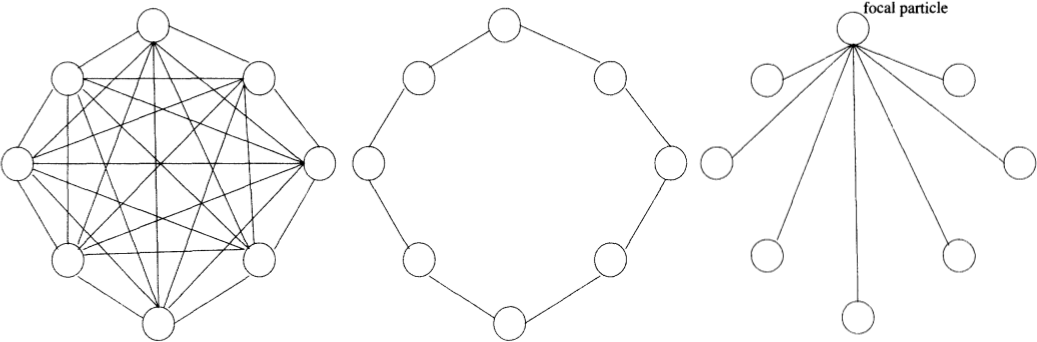
\includegraphics[width=\textwidth-\fboxrule-\fboxrule]{imgs/PSO.png}}
\end{figure}

\underline{Nota:} La vecidad se determina según \textbf{índices numéricos}, y no por medidas especiales (como la \textit{distancia euclídeana}, por ejemplo).

Los parámetros principales del PSO son la \textbf{velocidad máxima}, el \textbf{tamaño de la vecindad} y el \textbf{peso inercial}.

\subsubsection{Comparación con los algoritmos genéticos}

\begin{itemize}
\item Ambos usan reglas de transición \textbf{probabilíticas}.
\item Ambos están  basados en adaptación, pero en el PSO los cambios son obtenidos a través del aprendizaje entre iguales, no entre operadores de variación.
\item El PSO tiene memoria: las partículas guardan registro de las mejores soluciones, y las velocidades anteriores son usadas para ajustar posiciones.
\item El PSO no tiene función de \textit{fitness}: el proceso de búsqueda es guíado por interacciones sociales entre partículas.
\end{itemize}

\subsection{Colonias de Hormigas}

\subsubsection{Inspiración biológica}

La esencia de modelar colonias de hormigas es el encontrar un modelo matemático que describa de forma precisa las características de \textbf{estigmergía} (``\textit{invisible manager}'') correspondientes a cada individuo.

La \textbf{estigmergía artificial} está definida como la comunicación indirecta mediada por modificaciones numéricas de los estados ambientales que son solos localmente accesibles por los agentes comunicadores.

\subsubsection{Algoritmo básico}

\begin{enumerate}
\item Comportamiento inicial aleatorio.
\item Cuando encuentran una fuente de comida, se organizan y comienzan a seguir el nuevo camino.
\begin{enumerate}[2.1]
\item Mecanismo de reclutamiento: mayormente por \textbf{feromonas}, liberados al regresar.
\item Si otros encuentran el rastro, lo seguirán probablemente.
\item El rastro se refuerza al ser seguido por más hormigas (pero se va evaporando).
\end{enumerate}
\end{enumerate}

\section{Lo que le tomaron a Marcus}
SOM, logica difusa, y enjambre de particulas y q les cuente como funcionaba. El teorema de la entropia borrosa eso fue lo mas especifico q me preguntaron

\end{document}